\documentclass[12pt]{article}
\usepackage{graphicx}
\graphicspath{ {../art/} }

\renewcommand{\bottomfraction}{0.9}
\renewcommand{\topfraction}{0.9}

\addtolength{\textwidth}{1in}
\addtolength{\oddsidemargin}{-0.5in}
\addtolength{\textheight}{1.0in}
\addtolength{\topmargin}{-0.5in}
%\addtolength{\topmargin}{0in}

\newcommand{\bid}[1]{\mbox{\bf #1\/}}
\newcommand{\rid}[1]{\mbox{\rm #1\/}}
\newcommand{\tid}[1]{\mbox{\tt #1\/}}
\newcommand{\id}[1]{\mbox{\it #1\/}}
\newcommand*{\ngg}{\mathop{\neg}}
\newcommand*{\imp}{\mathbin{\rightarrow}}
\newcommand*{\revimp}{\mathbin{\leftarrow}}
\newcommand*{\eqv}{\mathbin{\leftrightarrow}}
\newcommand*{\neqv}{\mathbin{\oplus}}
\newcommand*{\logeqv}{\mathrel{\equiv}}
\newcommand*{\fml}{\mathit{fml}}


\begin{document}

\section*{Mutual Exclusion Proof}

\noindent Given Peterson's algorithm expressed as automata:

\vspace{1em}
\begin{figure}[h]
\centering
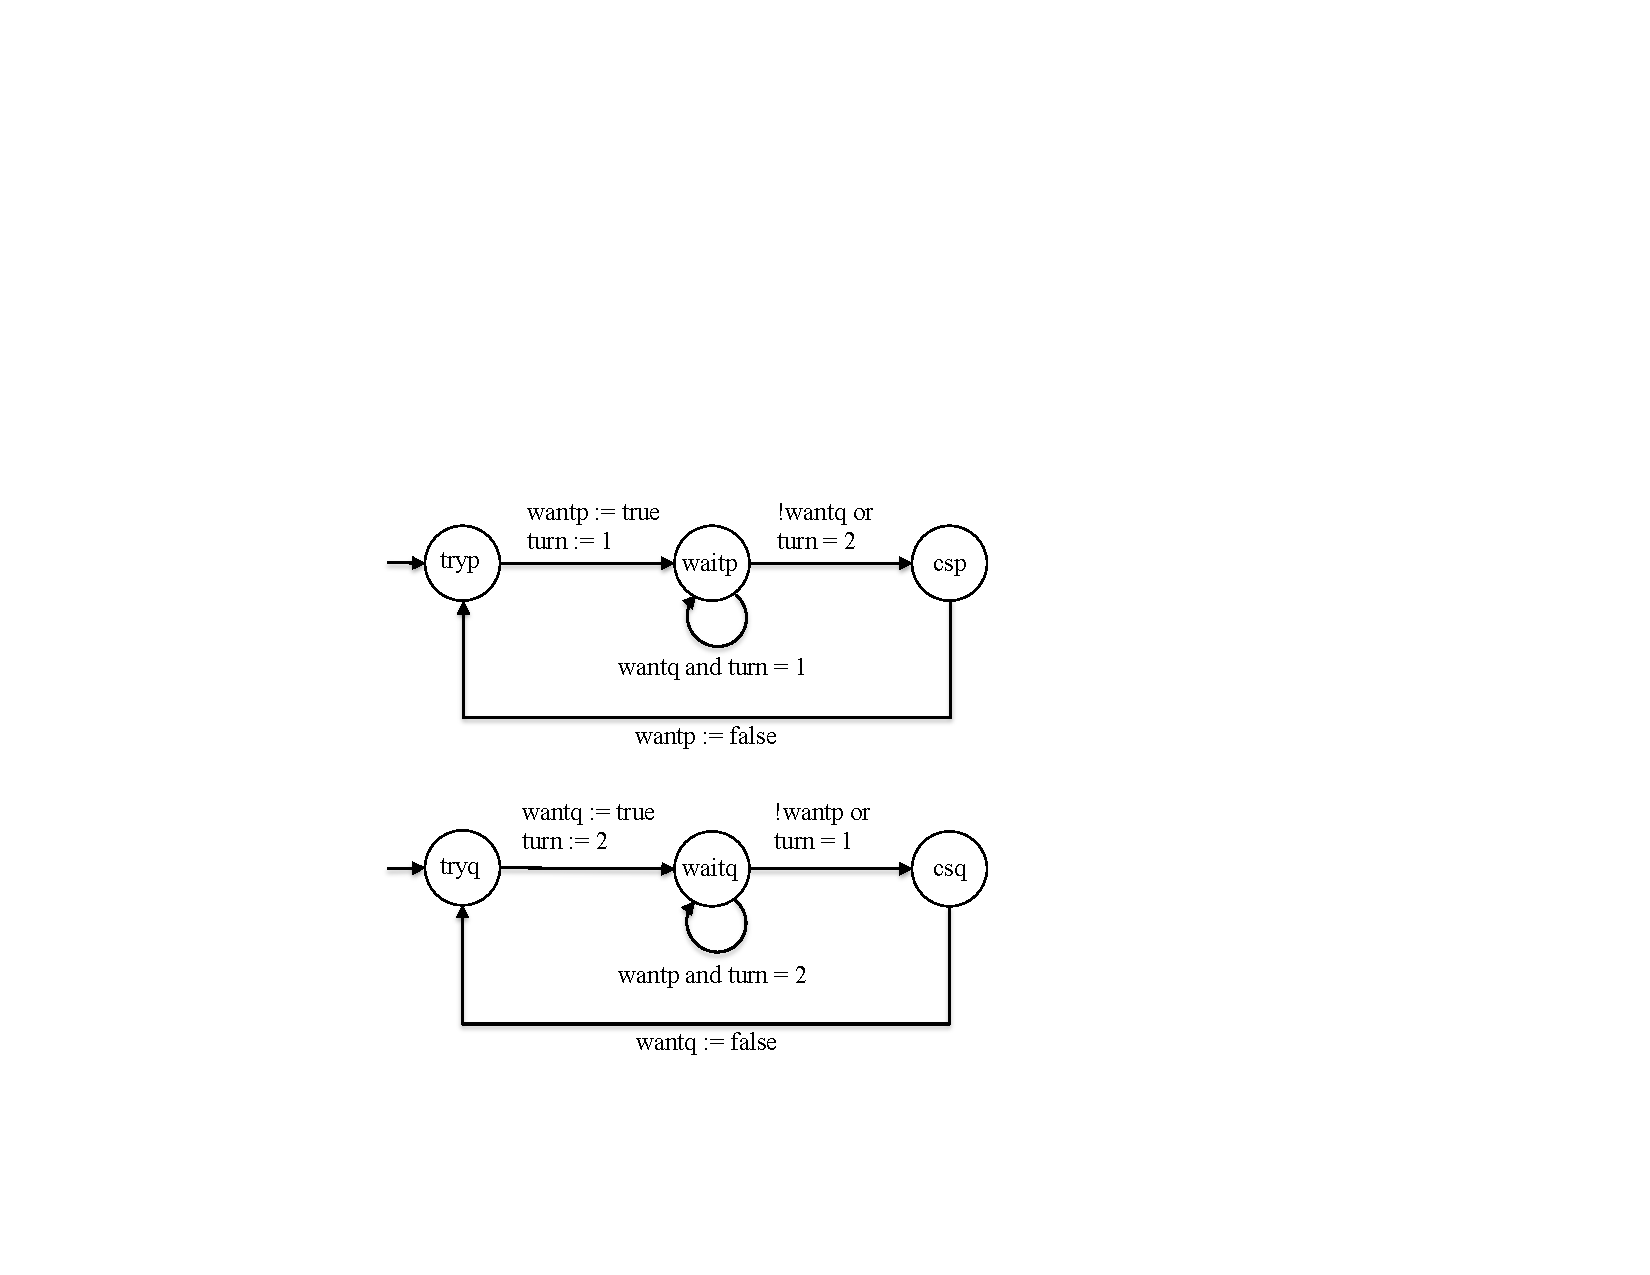
\includegraphics[width=4.0in, height=5.0in,keepaspectratio=true]{peterson.pdf}
\caption{Peterson's algorithm}
\label{pa}
\end{figure}
\noindent we wish to prove it guarantees mutually-exclusive access to critical sections
{\tt csp} and {\tt csq}, a kind of {\em safety\/} property.

\subsection*{Some facts}
\begin{enumerate}
\item A {\em state\/} of the algorithm's computation contains a location 
such as $\tid{tryq}$ or $\tid{waitp}$ and the values of $\tid{wantp}$, $\tid{wantq}$ and $\tid{turn}$.
Let $\id{Loc}_p=\{\tid{tryp},\tid{waitp},\tid{csp}\}$ and
$\id{Loc}_q = \{\tid{tryq},\tid{waitq},\tid{csq}\}$.
%A state is interpreted as a value of ($\id{location},\tid{wantp},\tid{turn}$).
%\item Automata make location in state unncessary.
%So state of $p,q\in\id{Bool}\times\{1,2\}$.

\item Each automaton has two types of transitions: those checking a condition and those guaranteeing one
through assignment statements.
We can convert assignments to conditions that we know will always be satisfied by virtue of the assignments
(e.g.\ {\tt wantp := true} becomes {\tt wantp = true}).

\item Each automaton has a
{\em transition function\/}: $\delta_p : \id{Loc}_p\times\id{state}\rightarrow\id{Loc}_p$
and $\delta_q : \id{Loc}_q\times\id{state}\rightarrow\id{Loc}_q$.
They allow one to ``run'' the automata on a given sequence of states.

\item $\delta_p$ and $\delta_q$ are {\em total\/} functions.
For any location at which no transition has a condition satisfied by a given state, the automaton remains
in that location.
%Each is defined at its locations 
%only for those states satisfying the condition required for a transition to occur at that location.
%The sequences of states for which both transition functions are defined at every state 
%in the sequence give the {\em semantics\/} of 
%Peterson's algorithm.
\end{enumerate}

\subsection*{A mutual exclusion theorem}

\noindent Define a multi-step version of a transition function $\delta$,
namely $\hat{\delta}$, as follows:

\[
\begin{array}{l}
\hat{\delta}(\id{loc},\epsilon) = \id{loc} \\
\hat{\delta}(\id{loc}, wa) = \delta(\hat{\delta}(\id{loc},w),a)
\end{array}
\]
where $\id{loc}$ is a location, $wa$ is a nonempty state sequence ending with state ``$a$''
and $\epsilon$ denotes the empty state sequence.

%\vspace{1em}
%\noindent
%Program $p$ expects states of the form $(\tid{wantp,turn})$ as inputs whereas $q$ expects
%states of the form $(\tid{wantq,turn})$.

%\vspace{1em}
%\noindent Interleaving execution of $p$ and $q$ to achieve concurrency requires introducing 
%a shared state.
%Each automaton shall therefore run on a sequence of states where each state represents one of
%eight values of $(\tid{wantp,wantq,turn})$.
%Call this sequence a {\em shared-state\/} sequence.

\vspace{1em}
\noindent {\em Mutual exclusion theorem}.
Let $\delta_p$ and $\delta_q$ be the transition functions derived for the automata
of Peterson's algorithm as given in Fig.\ref{pa}.
There's no state sequence $w$ such that $\hat{\delta}_p(\id{tryp},w)=\id{csp}$ and
$\hat{\delta}_q(\id{tryq},w)=\id{csq}$.

\vspace{1em}
\noindent The proof depends on the following Lemma:

\vspace{1em}
\noindent {\em Lemma}.
Suppose $w$ is a state sequence.  Then
\begin{enumerate}
%\item[(a)] $\hat{\delta}_p(\id{tryp},w)=\id{tryp}\wedge w\neq\epsilon \Rightarrow$ $w$ ends with $\neg\id{wantp}$.
\item[(a)] $\hat{\delta}_p(\id{tryp},w)=\id{waitp}\; \imp w$ ends with a
state in which $\id{wantp}$ holds.
\item[(b)] $\hat{\delta}_p(\id{tryp},w)=\id{csp}\; \imp w$ ends with a
state in which $(\neg\id{wantq}\vee\id{turn}=2)\wedge\id{wantp}$ holds.

%\item[(d)] $\hat{\delta}_q(\id{tryq},w)=\id{tryq}\wedge w\neq\epsilon \Rightarrow$ $w$ ends with $\neg\id{wantq}$.
\item[(c)] $\hat{\delta}_q(\id{tryq},w)=\id{waitq}\; \imp$ $w$ ends with a
state in which $\id{wantq}$ holds.
\item[(d)] $\hat{\delta}_q(\id{tryq},w)=\id{csq}\; \imp$ $w$ ends with 
a state in which $(\neg\id{wantp}\vee\id{turn}=1)\wedge\id{wantq}$ holds.
\end{enumerate}

\vspace{1em}
\noindent {\em Proof\/}.  The proof is by mutual induction on the length of $w$.
We show only (a) and (b) since (c) and (d) are handled similarly.

\vspace{0.5em}
{\em Basis\/}. $|w|=0$ or $w=\epsilon$.
(a) and (b) are vacuously true since $\hat{\delta}_p(\id{tryp},\epsilon)=\id{tryp}$, making
their antecedents false.

\vspace{1em}
{\em Inductive step\/}.
Suppose (a) and (b) hold for a state sequence $w$ where $|w|\geq 0$.
We show (a) and (b) hold for state sequence $wa$ where $a$ is the final state
in the sequence.

\begin{enumerate}
%\item[(a)]  Suppose $\hat{\delta}_p(\id{tryp},wa)=\id{tryp}$.
%Since $|wa|>0$, we have that $\hat{\delta}_p(\id{tryp},w)=\id{csp}$ and $\delta(\id{csp},a)=\id{tryp}$.
%And $\delta(\id{csp},a)=\id{tryp}$ only if $\neg\id{wantp}$ holds in $a$.

\item[(a)]  Suppose $\hat{\delta}_p(\id{tryp},wa)=\id{waitp}$.
There are two cases:
\begin{enumerate}
\item[1.]  $\hat{\delta}_p(\id{tryp},w)=\id{tryp}$ and $\delta_p(\id{tryp},a)=\id{waitp}$.
We have $\delta_p(\id{tryp},a)=\id{waitp}$ only if $\id{wantp}$ holds in $a$ by definition of $\delta_p$.
\item[2.]  $\hat{\delta}_p(\id{tryp},w)=\id{waitp}$ and $\delta_p(\id{waitp},a)=\id{waitp}$.
Nowhere in the automaton from which $\delta_q$ is derived is {\tt wantp} updated, nor is it
updated in the transition from {\tt waitp} to itself in the automaton from which $\delta_p$ is derived.
Therefore the value of {\em wantp\/} in $a$ is its value in the final state of $w$.
By induction and (a), {\em wantp\/} holds in the final state of $w$, hence it holds in $a$.
\end{enumerate}
\item[(b)]  Suppose $\hat{\delta}_p(\id{tryp},wa)=\id{csp}$.
We have $\hat{\delta}_p(\id{tryp},w)=\id{waitp}$ and $\delta_p(\id{waitp},a)=\id{csp}$.
And $\delta_p(\id{waitp},a)=\id{csp}$ only if $\neg\id{wantq}\vee\id{turn}=2$ holds in $a$ by definition
of $\delta_p$.
Further, nowhere in the automaton from which $\delta_q$ is derived is {\tt wantp} updated, nor is it
updated in the transition from {\tt waitp} to {\tt csp} in the automaton from which $\delta_p$ is derived.
Therefore the value of {\em wantp\/} in $a$ is its value in the final state of $w$.
By induction and (a), {\em wantp\/} holds in the final state of $w$, hence it holds in $a$.
\end{enumerate}
\noindent {\em End proof\/}.

\vspace{1em}
\noindent {\em Proof of mutual exclusion theorem\/}.
Suppose there is a state sequence $w$ such that $\hat{\delta}_p(\id{tryp},w)=\id{csp}$
and $\hat{\delta}_q(\id{tryq},w)=\id{csq}$.
Then by the preceding Lemma, $w$ must end with a state in which
\[(\neg\id{wantq}\vee\id{turn}=2)\wedge\id{wantp}\;\wedge\;
(\neg\id{wantp}\vee\id{turn}=1)\wedge\id{wantq}
\]
holds. This formula is only satisfiable if unit literals $\id{wantp}$ and
$\id{wantq}$ are true, which implies $\id{turn}=1\wedge\id{turn}=2$, a contradiction.
\end{document}
